\chapter{Beam Use Proposal 2023--2025}
\label{chap:beam_use_proposal}

In this Chapter we detail the sPHENIX Beam Use Proposal as requested
in the Associate Laboratory Director Charge for three years of running
during the period 2023--2025 assuming 24 or 28 cryo-weeks in each
year.  The complete charge is reproduced in
Appendix~\ref{chap:charge}.

\section{Years 2023--2025 Proposal}

The three-year proposal is summarized in Table~\ref{tab:summary}.   The numbers correspond to 24-cryo weeks in each year with alternate numbers in parenthesis corresponding to 28-cryo weeks.    The recorded luminosity values correspond to events collected via minimum bias triggers that sample a large fraction of the inelastic cross section ($> 90\%$ in Au+Au for example).    These events have collision vertex $|z|<10$~cm that corresponds to the optimal acceptance range for the full sPHENIX detector, including the inner tracker.    

%The sPHENIX inner vertex tracker MVTX is detailed in sPH-HF-2018-001 [\url{https://indico.bnl.gov/event/4072/}].   The MVTX consists of three layers with active ladder length of 271.2~mm or $\pm135.6$~mm at an average radius of 25.2, 33.4, and 41.5~mm, respectively. Therefore, collisions taking place within $|z| < 10$~cm will have optimal acceptance of $|\eta| < 1.0$ if one requires all tracks in this $\eta$ range to pass through at least two layers of the MVTX.

In 2024, we include two sets of values, with the first corresponding to simply recording 5~kHz of minimum bias data in \pp and \pau collisions.   The second value is with minor data acquisition upgrade for partial streaming readout (10\%-$str$) for the Time Projection Chamber (TPC) and the inner tracking detectors (MVTX, INTT).    Thus, these recorded luminosities are for the tracking detectors only, i.e. without the calorimeters.   Details on the streaming readout upgrade are given in Chapter~\ref{chap:readout}.
The sampled luminosity values correspond to additional events that are efficiently sampled with physics specific Level-1 triggers with trigger efficiencies greater than 90\%.    In this document we detail specifically which physics channels are enhanced from these Level-1 triggers.     

\begin{table}[]
\centering
\caption{
Summary of sPHENIX Beam Use Proposal for the years
  2023--2025, as requested in the charge.  The values correspond to 24 cryo-week scenarios, while those in parentheses correspond to 28 cryo-week scenarios.    The 10\%-$str$ values correspond to a streaming readout of the tracking detectors.
  Full details are provided in
  Chapter~\ref{chap:beam_use_proposal}.
\label{tab:summary}}
\bigskip
\centering
\begin{tabular}{ | c | c | c | c | c | c | c | }
\hline
Year & Species & $\sqrt{s_{NN}}$ & Cyro  & Physics & Rec. Lum. & Samp. Lum. \\
     &         & [GeV]           & Weeks & Weeks   & $|z|<$10~cm & $|z|<$10~cm \\ \hline \hline

2023 & \auau   & 200 & 24 (28) & 9 (13) & 3.7 (5.7) \nb   & 4.5 (6.9) \nb  \\ \hline \hline 
2024 & $p^{\uparrow}p^{\uparrow}$     & 200 & 24 (28) & 12 (16) & 0.3 (0.4) \pb [5 kHz] & 73 (101) \pb  \\
     &                                &     &  & &  7.3 (10.1) \pb [10\%-$str$]&   \\ \hline
2024 & $p^{\uparrow}$+Au    & 200 & -- & 5 & 0.003 \pb [5 kHz]          & 0.11 \pb \\  
 &     &  &  &  &  0.01 \pb [10\%-$str$]         &   \\ \hline \hline
2025 & \auau   & 200 & 24 (28) & 20.5 (24.5) & 13 (15) \nb   & 21 (25) \nb  \\ \hline

\end{tabular}

\end{table}

The first year 2023 of running has significant commissioning time for the detector, and critically for the accelerator-detector combination, as expected for any new major, complex collider experiment.   It is critical that this commissioning time be with \auau collisions at 200 GeV to insure a full understanding of the detector operation and performance under high occupancy conditions.   Details on the commissioning plan are given in Chapter~\ref{chap:commissioning}.    After the commissioning period, 9 (13) weeks of physics data taking are available corresponding to recorded \auau minimum bias data sets of 25 (39) billion events.   The main \auau physics run is in the third year, 2025, with more than 113 (141) billion events recorded in total for 2023 and 2025 running combined.
Note that for all the luminosity projections and conversions to collision rates we utilize as total inelastic cross sections:   6.8 barns, 1.7 barns, 42 millibarns for \auau, \pau, and \pp, respectively.

The second year, 2024, of running provides the critical baseline measurements in \pp and \pau both at $\sqrt{s_{NN}}=200$~GeV.   The proton beam in both cases will be with transverse (vertical) polarization.  These data sets provide key baseline measurements for nuclear modification factors R$_{AA}$, R$_{pA}$, new collectivity and probes of small collision systems, as well as compelling transverse spin physics observables.    We highlight that particularly in this year, the 24 cryo-week scenario is challenging since new Level-1 triggers will be commissioned and C-AD requires a significant number of cryo-weeks for switching systems.    

In the following sections, we detail the running conditions worked out with the Collider-Accelerator Division (C-AD) experts.    We then provide detailed cryo-week breakdowns for each running year, along with explicit assumptions for calculating the recorded and sampled luminosities.   

Specific details on the RHIC luminosity projections, mapping out of cryo-weeks schedules, and overall trigger/sampling calculations are given in the next Sections.

\section{RHIC Luminosity Projections}

%For planning purposes in this document, we use luminosity projection numbers provided by C-AD.   The version of the document titled ``RHIC Collider Projections (FY 2017 –- FY 2027)'' utilized for this study is dated 21 August 2020 and uses knowledge gained from the Run-15 \pp and \pAu at 200~GeV running and the Run-16 \auau at 200 GeV running.   The document is available at:

%\vspace{0.1in}
%{\color{blue}{http://www.rhichome.bnl.gov/RHIC/Runs/RhicProjections.pdf}} 
%\vspace{0.1in}

%The document linked above is periodically updated, so note the date tag.  In general, C-AD provides a minimum and maximum luminosity per week for each running period, as well as the fraction of collisions within a given z-vertex range. For calculating the integrated luminosity, we assume a ramp-up curve and then a steady-state physics running at the mean of the minimum and maximum in both luminosity and z-vertex fraction within $|z|<$10~cm (where a minimum and maximum are given).  The C-AD minimum and maximum projections are fully detailed in the document linked above.

The detailed C-AD inputs are described in Chapter~\ref{chap:cad}.
A critical part of the sPHENIX run plan is to have a non-zero crossing angle between the beams.    We detail the crossing angle reasoning, implications, and quantitative analysis in Chapter~\ref{chap:cad}.    

For this plan, we assume an sPHENIX up-time (i.e. the fraction of time when collisions are available when sPHENIX is taking data with high livetime) of 0.60 for the first two years of running (2023 and 2024) since the detector is being commissioned for new collision systems and new Level-1 triggers are being brought online, and 0.80 for subsequent running (2025).   These up-time values fold in the expected deadtime of the data acquisition system, which is greater than 90\%.

RHIC C-AD projections for time in store (i.e. RHIC up-time) vary slightly with most of the projected values around 0.60. It is notable that C-AD projections are for a nominal 8 hour store; however, a more optimal store length may be found in future running at closer to 5 hours.

\section{Cryo-Weeks}

For mapping out a run plan, we state both cryo-weeks for a running period and also physics data taking weeks, i.e. when Physics Running is declared by C-AD.   The guidance from C-AD is that there is a 0.5 week ``cool down from 50 K to 4 K'', then a 2.0 week ``set-up mode'' for the specific collision species, and then a 0.5 week ``ramp-up''.   If switching species, there is again a 2.0 week ``set-up'' and 0.5 week ``ramp-up''.    Lastly, at the end of the running period, there is a 0.5 ``warm-up from 4 K to 50 K''.  
In addition, we assume that in the first, second and third weeks of declared Physics Running, one achieves 25\%, 50\%, and then 75\% of the luminosity target, with subsequent weeks at 100\%.  These are standard assumptions following C-AD guidance.

Following said C-AD guidance, we present the cryo-week break downs for the 24 (28) week scenarios.   
The break-downs are shown for 2023 in Table~\ref{tab:cryoplan2023}, for 2024 in Table~\ref{tab:cryoplan2024}, and for
2025 in Table~\ref{tab:cryoplan2025}.

\begin{table}
\centering
\begin{tabular}{ | c | l | }
\hline
Weeks & Designation \\ \hline
0.5  & Cool Down from 50 K to 4 K \\ \hline
2.0  & Set-up mode 1 (Au+Au at 200 GeV) \\ \hline
0.5  & Ramp-up mode 1 (8 h/night for experiments) \\ \hline
11.5  & sPHENIX Initial Commission Time \\ \hline
9.0 (13.0) & Au+Au Data taking (Physics) \\ \hline
0.5  & Controlled refrigeration turn-off \\ \hline \hline \hline
24.0 (28.0) & Total cryo-weeks \\
\hline
\end{tabular}
\caption{Year 2023 run plan for 24 (28) cryo-weeks with \auau 200~GeV collisions.\label{tab:cryoplan2023}}
\end{table}

\begin{table}
\centering
\begin{tabular}{ | c | l | }
\hline
Weeks & Designation \\ \hline
0.5  & Cool Down from 50 K to 4 K \\ \hline
2.0  & Set-up mode 1 (p$^{\uparrow}$p$^{\uparrow}$ at 200 GeV) \\ \hline
0.5  & Ramp-up mode 1 (8 h/night for experiments) \\ \hline
12.0 (16.0) & Data taking mode 1 (p$^{\uparrow}$p$^{\uparrow}$ Physics) \\ \hline
1.0  & Move DX magnets \\ \hline
2.0  & Set-up mode 2 (p$^{\uparrow}$+Au at 200 GeV) \\ \hline
0.5  & Ramp-up mode 2 (8 h/night for experiments) \\ \hline
5.0 & Data taking mode 2 (p$^{\uparrow}$+Au Physics) \\ \hline
0.5  & Controlled refrigeration turn-off \\ \hline \hline \hline
24.0 (28.0) & Total cryo-weeks \\
\hline
\end{tabular}
\caption{Year 2024 run plan for 24 (28) cryo-weeks with p$^{\uparrow}$p$^{\uparrow}$ and p$^{\uparrow}$+Au 200~GeV collisions.\label{tab:cryoplan2024}}
\end{table}

\begin{table}
\centering
\begin{tabular}{ | c | l | }
\hline
Weeks & Designation \\ \hline
0.5  & Cool Down from 50 K to 4 K \\ \hline
2.0  & Set-up mode 1 (Au+Au at 200 GeV) \\ \hline
0.5  & Ramp-up mode 1 (8 h/night for experiments) \\ \hline
20.5 (24.5) & Au+Au Data taking (Physics) \\ \hline
0.5  & Controlled refrigeration turn-off \\ \hline \hline \hline
24.0 (28.0) & Total cryo-weeks \\
\hline
\end{tabular}
\caption{Year 2025 run plan for 24 (28) cryo-weeks with \auau 200~GeV collisions.\label{tab:cryoplan2025}}
\end{table}

\section{Sampled versus Recorded Luminosity}

In the \auau 200~GeV case, the physics will predominately come from {\bf recorded} minimum bias collisions.   This data will be selected by the Level-1 trigger via the MBD that samples approximately 90\% of the inelastic cross section.   Additional physics may be ``sampled'' with rare event triggers, for
example high-\pt direct photons, where the trigger rejection is very high even in central \auau events.   All physics projections are based on the recorded luminosity in \auau unless otherwise stated.     
The key requirements to achieve these recorded event sets are (1) the sPHENIX Data Acquisition Level-1 accept rate of 15~kHz with livetime greater than 90\%, (2) the luminosity corresponds to a rate of collisions within $|z|<10$~cm during the store above 15~kHz, and (3) maintaining the sPHENIX and RHIC uptime projections. 
As shown in Figure~\ref{fig:auaulumcurves}, the projected \auau collision rate within $|z|<10$~cm exceeds the 15~kHz minimum bias recording capacity for most all of a five-hour store.   There is a factor of order 1.5, depending on the year, that can be additionally sampled by very selective physics triggers in \auau even at the lower luminosity selection.

\begin{figure}
\centering
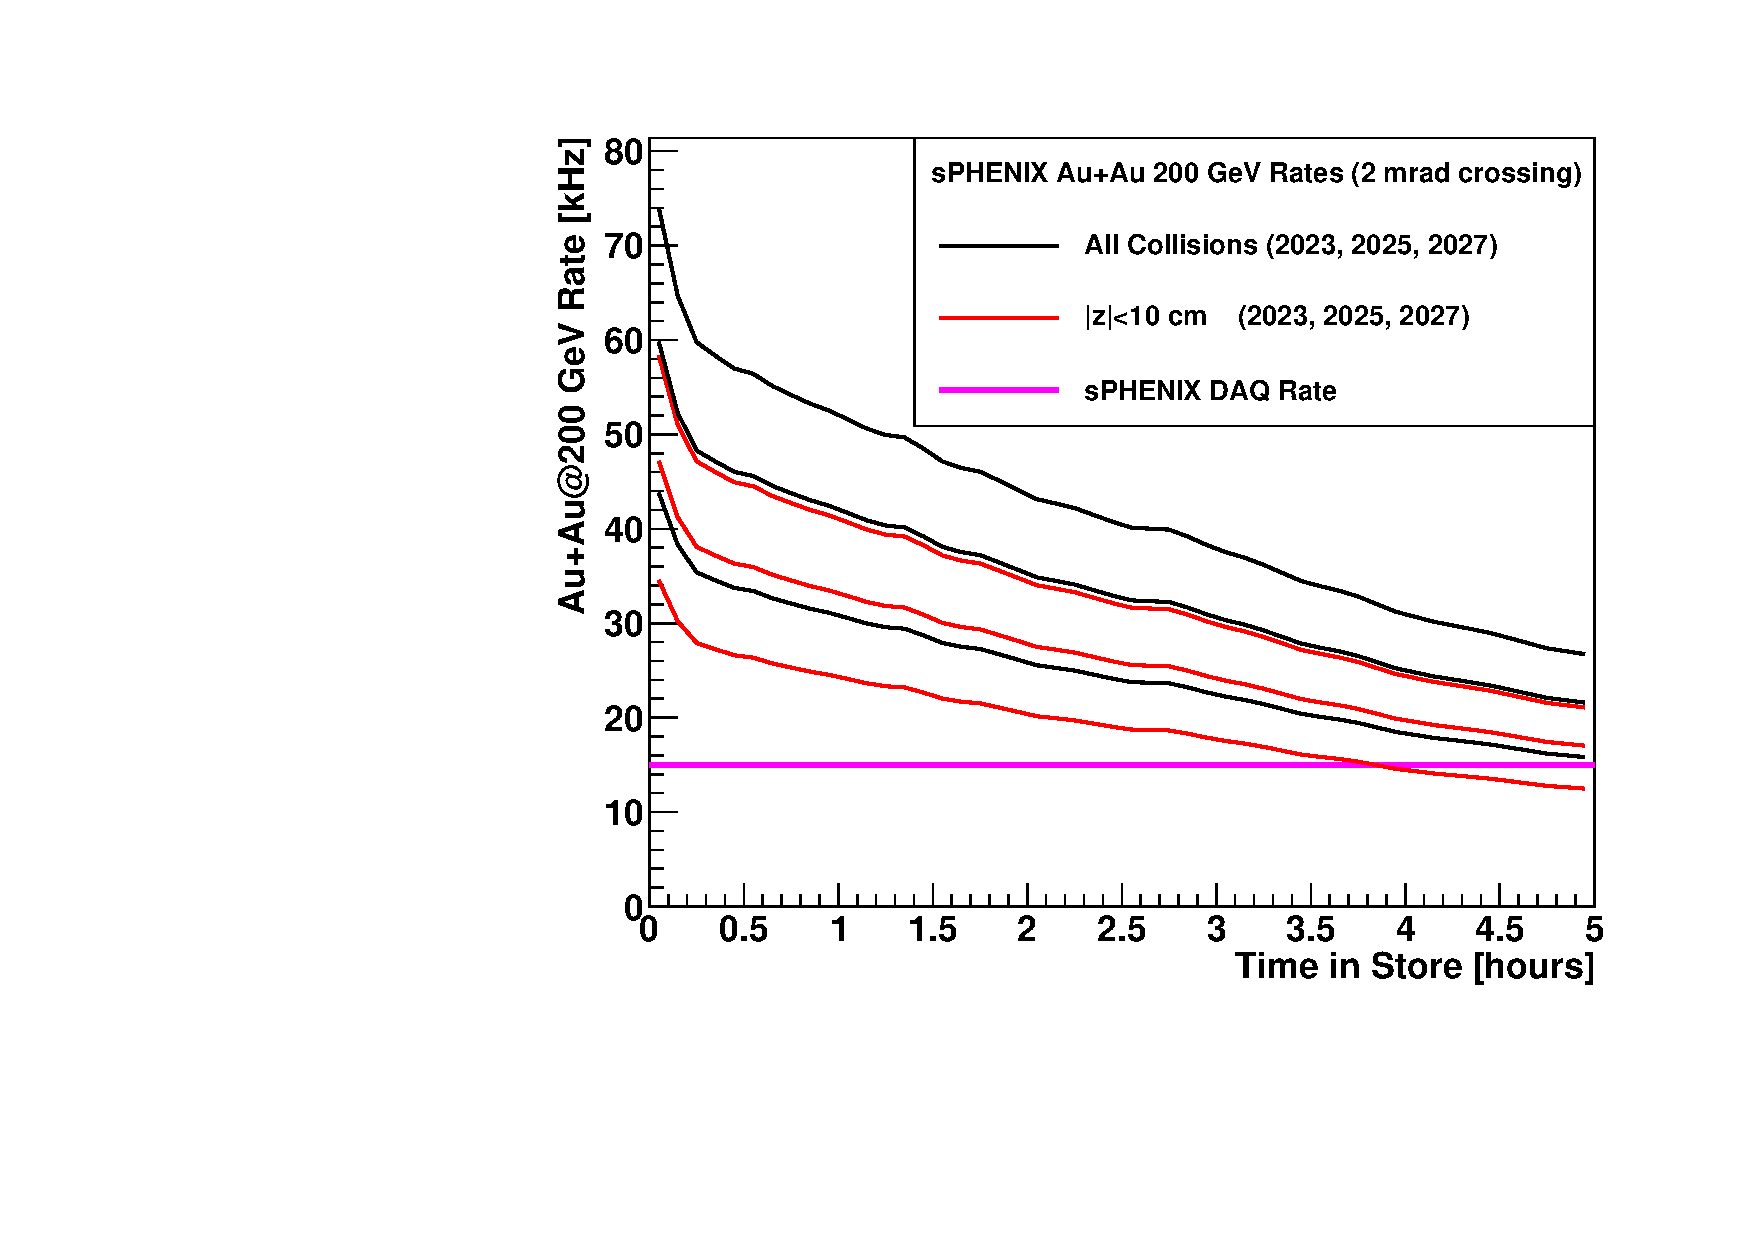
\includegraphics[width=0.70\linewidth]{figs/figure_auauratestore_2mrad.pdf} 
\caption{Estimated \auau at 200~GeV collision rate as a function of Time in Store for all collisions (black) and collisions within $\pm$10~cm (red).  The bottom to top set of curves in each color are for the mean luminosity and fraction within $\pm$10~cm for the C-AD projections labeled in their document as 2023, 2025, 2027, with the maximum projections for 2025 and 2027.   Also shown as a magenta line is the sPHENIX Data Acquisition Level-1 accept rate of 15~kHz for reference.
\label{fig:auaulumcurves}}
\end{figure}

In the \pp and \pau case, the physics will predominantly come from {\bf sampled} Level-1 triggered events utilizing photon, electron (e.g. from Upsilon decays), hadron, and
jet triggers.  Thus, the key value is the sampled luminosity for these physics channels.   Note that some observables such as lower \pt hadrons (and in particular heavy-flavor hadrons $D$, $\Lambda_{c}$, $B$) do not have effective Level-1 physics triggers.    Thus, in these cases the recorded luminosity is crucial.    We have nominally allocated 5~kHz, out of the 15~kHz Level-1 trigger rate, for \pp and \pau minimum bias collection.   A critical addition is the streaming capability for the tracking detectors, which enables much larger minimum bias data sets (without calorimeter readout).

Trigger algorithms have been developed and tested for \pp and \pau running using the EMCal for single photons (typically with \pt greater than 10 GeV) and for electrons (from Upsilon decays typically with \pt greater than 3--4 GeV).  In addition, trigger algorithms using the combined EMCal and HCal information have been developed for selecting jets and single hadrons.    At the highest \pp interaction rates, rejection factors of order 5000--10,000 are needed to result in a 1--2~kHz bandwidth allocation for a given trigger channel.    Full {\textsc{GEANT-4}} simulations with {\textsc{HIJING}} \pp and \pau events have been used to document the trigger efficiencies and rejection factors for all Level-1 algorithms.
One example set of calculations for jet triggers is shown in Figure~\ref{fig:trigger} indicating good efficiency and rejection factors above the required level.

\begin{figure}
    \centering
    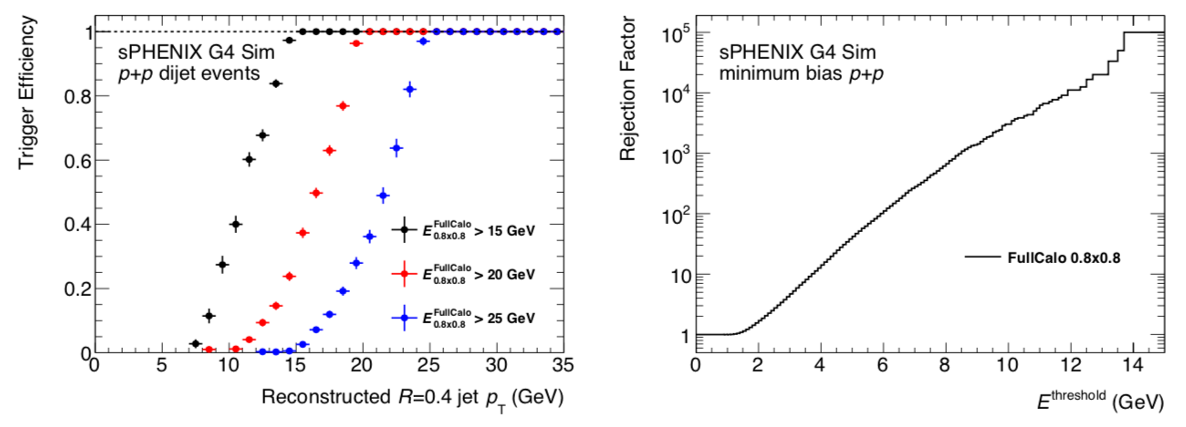
\includegraphics[width=\linewidth]{figs/figure_sphenix_jettrigger.png}
    \caption{sPHENIX full {\textsc{GEANT-4}} simulations with {\textsc{HIJING}} \pp events run through the jet Level-1 trigger emulator with efficiencies (left) and rejection factors (right).}
    \label{fig:trigger}
\end{figure}

%It is useful to put the data sets for the three proposed systems (\pp, \pau, \auau) into context, and so we compare the relative statistics for high $p_T$ jets.

Table~\ref{tab:ncoll} details the number of relevant events recorded or sampled for measuring high $p_T$ jets from running in 2023--2025.    
For \auau minimum bias events, the average number of binary collisions is 
$\left< N_{coll} \right> \approx 250$.   
Similarly, for \pau the $\left< N_{coll} \right> = 4.7$.
We note that the \auau sample with an order of magnitude more effective \pp collisions sampled will be divided into multiple centrality bins and jet quenching will reduce the statistics at high $p_T$.   This is a reasonable balance of cold and hot system measurements.

\begin{table}[]
    \centering
    \begin{tabular}{|c|c|c|c|}\hline
         Species & Year 1--3 Total & $\left< N_{coll} \right>$ & Effective-\pp \\ \hline\hline
         \pp & 62~\pb (sampled) & 1 & $2.4 \times 10^{12}$\\ \hline
         \pau & 0.11~\pb (sampled) & 4.7 & $0.9 \times 10^{12}$ \\ \hline
         \auau & 20.7~\nb (recorded) & 250 & $35 \times 10^{12}$ \\ \hline
    \end{tabular}
    \caption{Comparison from the full data sets from Years 2023--2025 assuming the 28 cryo-week scenarios for the three systems \pp, \pau, \auau.}
    \label{tab:ncoll}
\end{table}

 






